\section{Confiabilidad e integración del sistema}

Es la probabilidad de que el sistema desempeñe sus funciones dentro de los índices de desempeño requeridos. 

Para determinar la confiabilidad de componentes que se encuentren en serie se aplica
\[
    R_(T) = R_{1} \times R_{2} \times \cdots \times R_{i} \text{ \;\;\; \( i = 1, \cdots, n \) }
\]

Donde \( n \) es la cantidad de componentes en serie. Gráficamente se expresan como

\begin{figure}[h!]
    \centering
        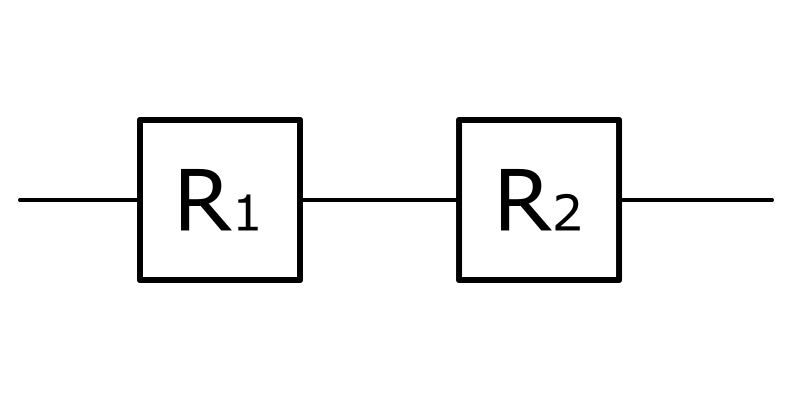
\includegraphics[scale=0.20]{Proyecto Integrador Figuras/24 Confiabilidad Serie.png}
        \caption{Confiabilidad en serie}
\end{figure}

Por ejemplo, un sistema de engranes montados a un eje, determine confiabilidad del sistema.

Para determinar la confiabilidad de los componentes que están en paralelo se aplica
\[
    R_{T} = 1 - (1 - R_{1}) (1 - R_{2}) \cdots (1 - R_{i}) \text{ \;\;\; \( i = 1, \cdots, n \)}
\]

Donde \( n \) es la confiabilidad de componentes en paralelo, gráficamente se expresa como

\begin{figure}[h!]
    \centering
        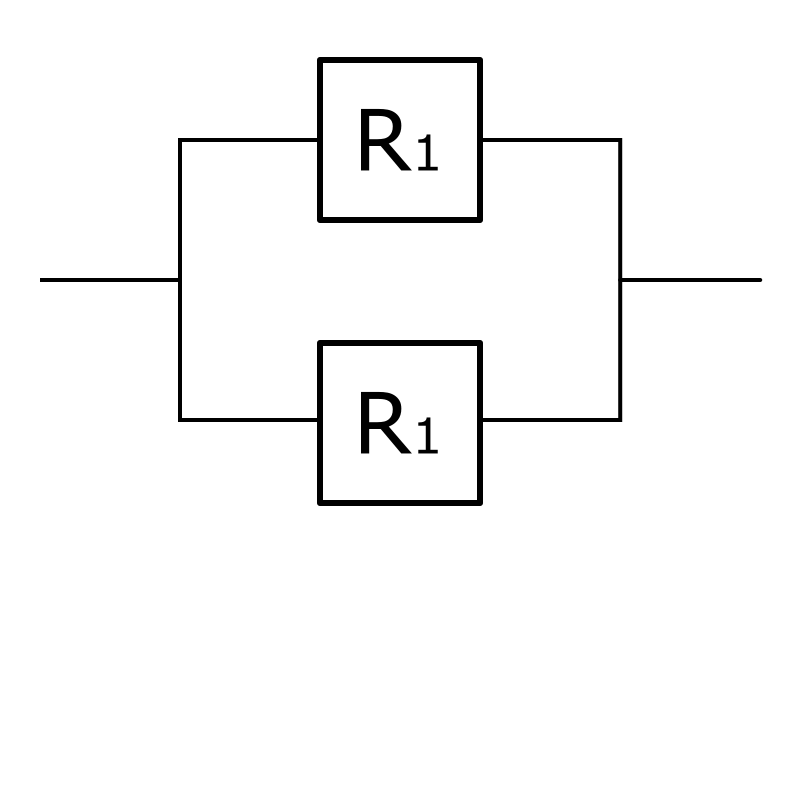
\includegraphics[scale=0.20]{Proyecto Integrador Figuras/25 Confiabilidad Paralelo.png}
        \caption{Confiabilidad en paralelo}
\end{figure}

\subsection{Integración del sistema}
La integración en el proceso de diseño mecatrónico es fundamental ya que tiene como propósito asegurar el comportamiento del sistema dentro de un rendimiento deseado, es decir, se busca que cada una de las partes del sistema operen de forma armónica. 

El proceso de integración también debe ser jerárquico, va integrando los componentes hasta volverse módulos, y posteriormente integra los módulos para convertirse en sistemas, y finalmente en el sistema mecatrónico. 

\begin{figure}[h!]
    \centering
        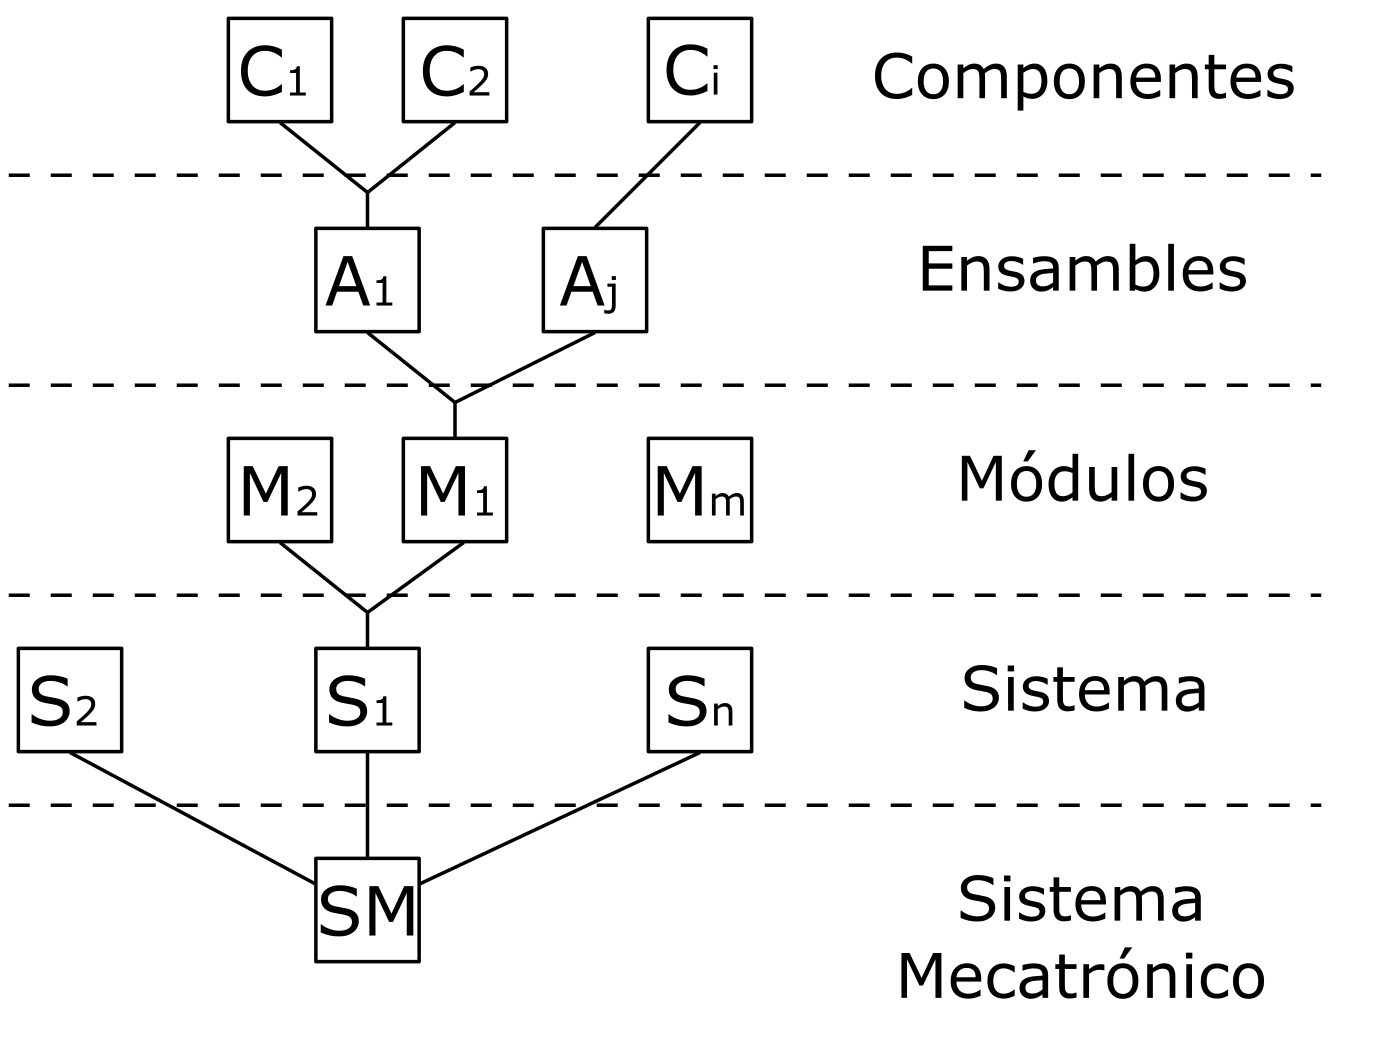
\includegraphics[scale=0.12]{Proyecto Integrador Figuras/26 Integracion del Sistema.png}
        \caption{Integración del sistema}
\end{figure}

El proceso de integración se divide en
\begin{enumerate}
    \item Integración de hardware: es la unión entre cada uno de los componentes físicos, son conexiones físicas, unión mecánica, contacto. 
    
    \item Integración de software: es la unión de componentes a través de información o energía, por ejemplo, algoritmo, control, protocolo, comunicación.
\end{enumerate}

En el proceso de integración es necesario diseñar nuevos componentes y/o modificar existentes para asegurar la integración armónica. 